\documentclass[12pt]{article}


\usepackage{amssymb}
\usepackage{amsmath}
\usepackage{fullpage}
\usepackage{epsfig}
\usepackage{epstopdf}

\newif\ifans

\anstrue

\begin{document}

\begin{center}
\underline{\LARGE{Chapter 2.1 Practice Problems}}
\end{center}

\noindent EXPECTED SKILLS:

\begin{itemize}

\item Be able to compute the average rate of change of a function over an interval; i.e., be able to find the slope of the secant line through two points on the graph of a function.

\item Be comfortable using a limit to compute the instantaneous rate of change of a function (for arbitrary and specific values); i.e., know how to find the slope of the tangent line to a function.

\end{itemize}

\noindent PRACTICE PROBLEMS:

\medskip

\begin{enumerate}

\item Find the average rate of change of the given function on the given interval.

\begin{enumerate}

\item $f(x) = x^2$ on $[0,2]$ 

\ifans{\fbox{2}} \fi

\item $f(x) = x^3-3x+5$ on $[-2,2]$ 

\ifans{\fbox{1}} \fi

\item $\displaystyle f(x) = \frac{1}{x}$ on $[1,2]$ 

\ifans{\fbox{$\displaystyle -\frac{1}{2}$}} \fi

\end{enumerate}

\item Find the instantaneous rate of change of the given function at the given point. 

\begin{enumerate}

\item $f(x) = x^2-1$ at $x=3$

\ifans{\fbox{6}} \fi

\item $f(x) = x^3$ at $x=2$ 

\ifans{\fbox{12}} \fi

\item $f(x)=\sqrt{x}$ at $x=9$

\ifans{\fbox{$\displaystyle \frac{1}{6}$}} \fi

\item $\displaystyle f(x) = \frac{1}{x^2}$ at $x=1$ 

\ifans{\fbox{$-2$}} \fi

\end{enumerate}

\newpage

\item A ball is thrown straight up in the air (from the ground) and its position in feet above the ground after $t$ seconds is given by: $f(t) = -8t^2+16t$. Answer the following questions about the path of the ball. 

\begin{enumerate}

\item  At what time $t$ does the ball hit the ground? 

\ifans{\fbox{After $2$ seconds}} \fi

\item What is the average velocity of the ball from $t=0$ to $t=1$? 

\ifans{\fbox{8 ft/sec}} \fi

\item What is the instantaneous velocity of the ball at $t=1$ second?

\ifans{\fbox{0 ft/sec}} \fi 

\item Below is the graph of $f(t)$.  Sketch the secant line whose slope is the average velocity of the ball on $[0,1]$.\\

\begin{center}
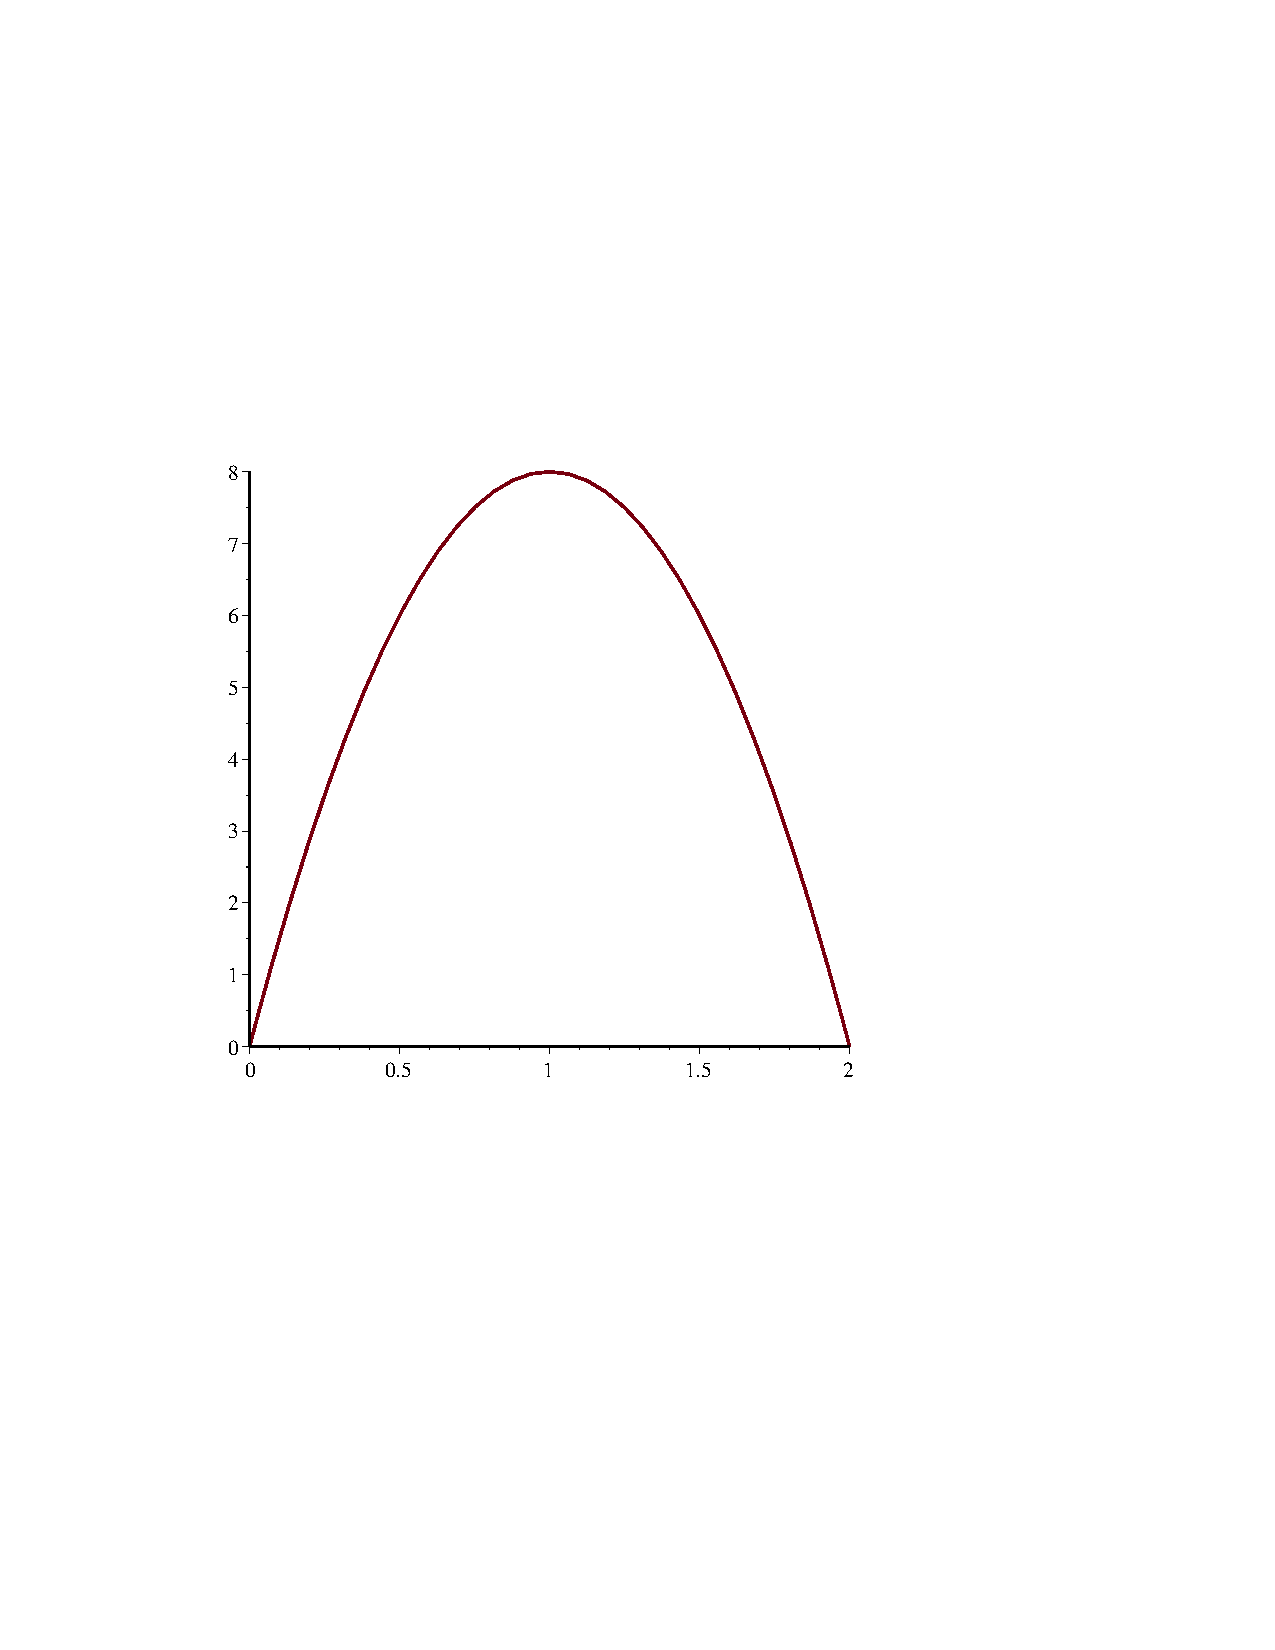
\includegraphics[scale=0.5]{graph2.pdf}
\end{center} 

\ifans{\fbox{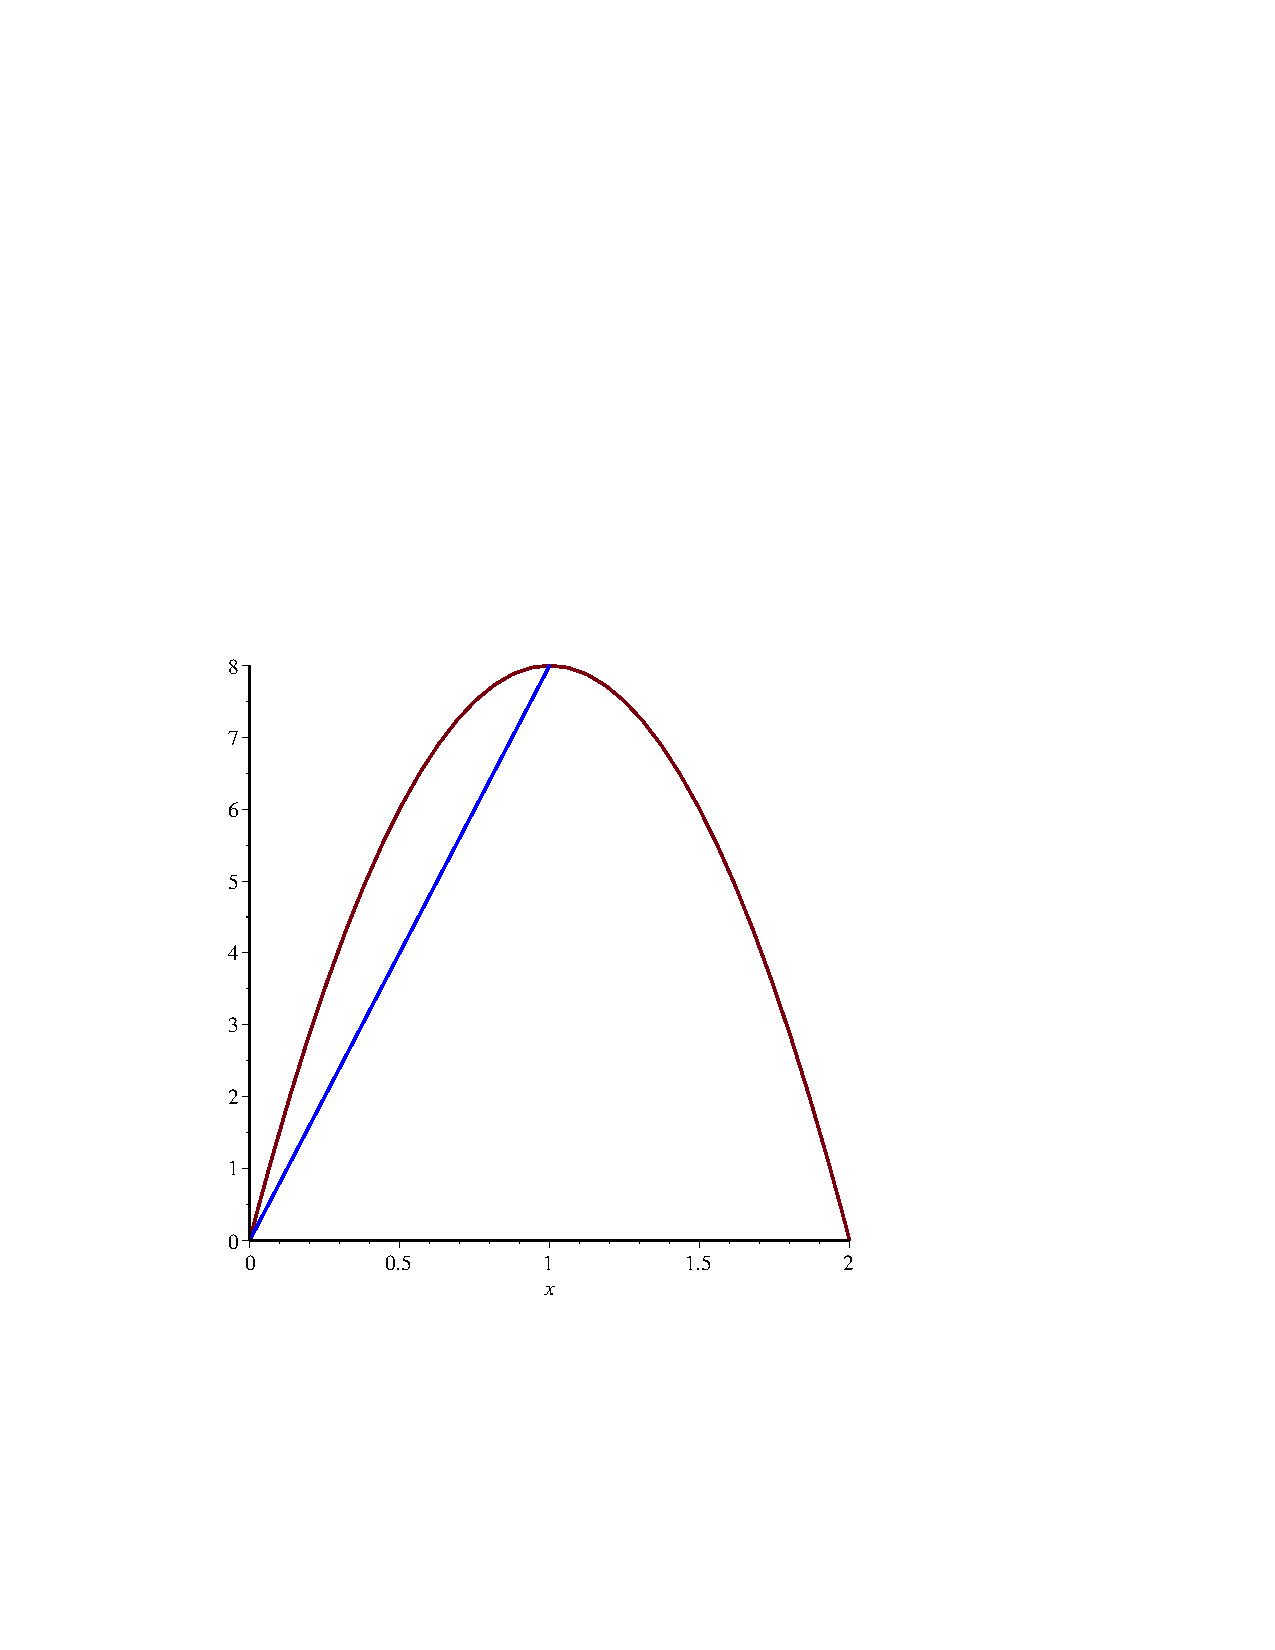
\includegraphics[scale=0.5]{graph3.pdf}}} \fi

\newpage

\item Below is the graph of $f(t)$.  Sketch the tangent line whose slope is the instantaneous velocity of the ball at $t=1$ second.\\

\begin{center}
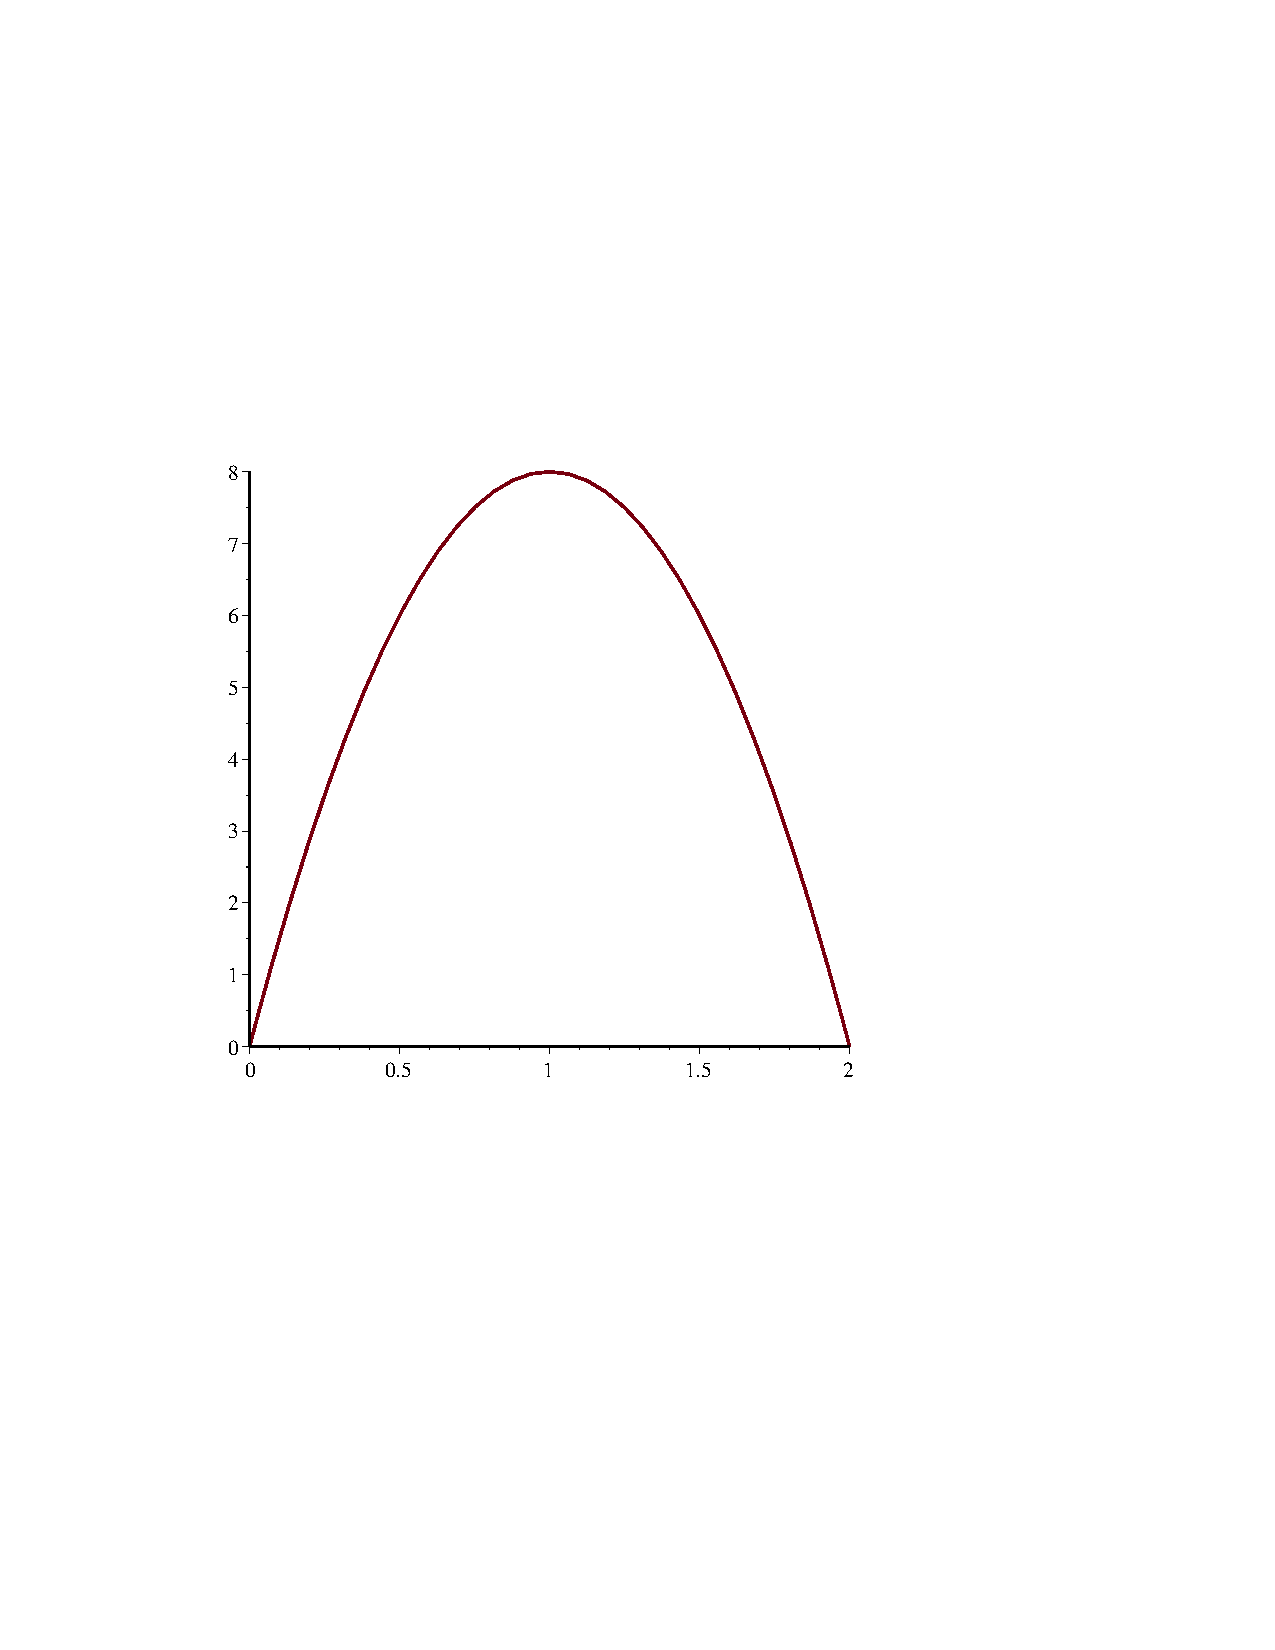
\includegraphics[scale=0.5]{graph2.pdf}
\end{center}

\ifans{\fbox{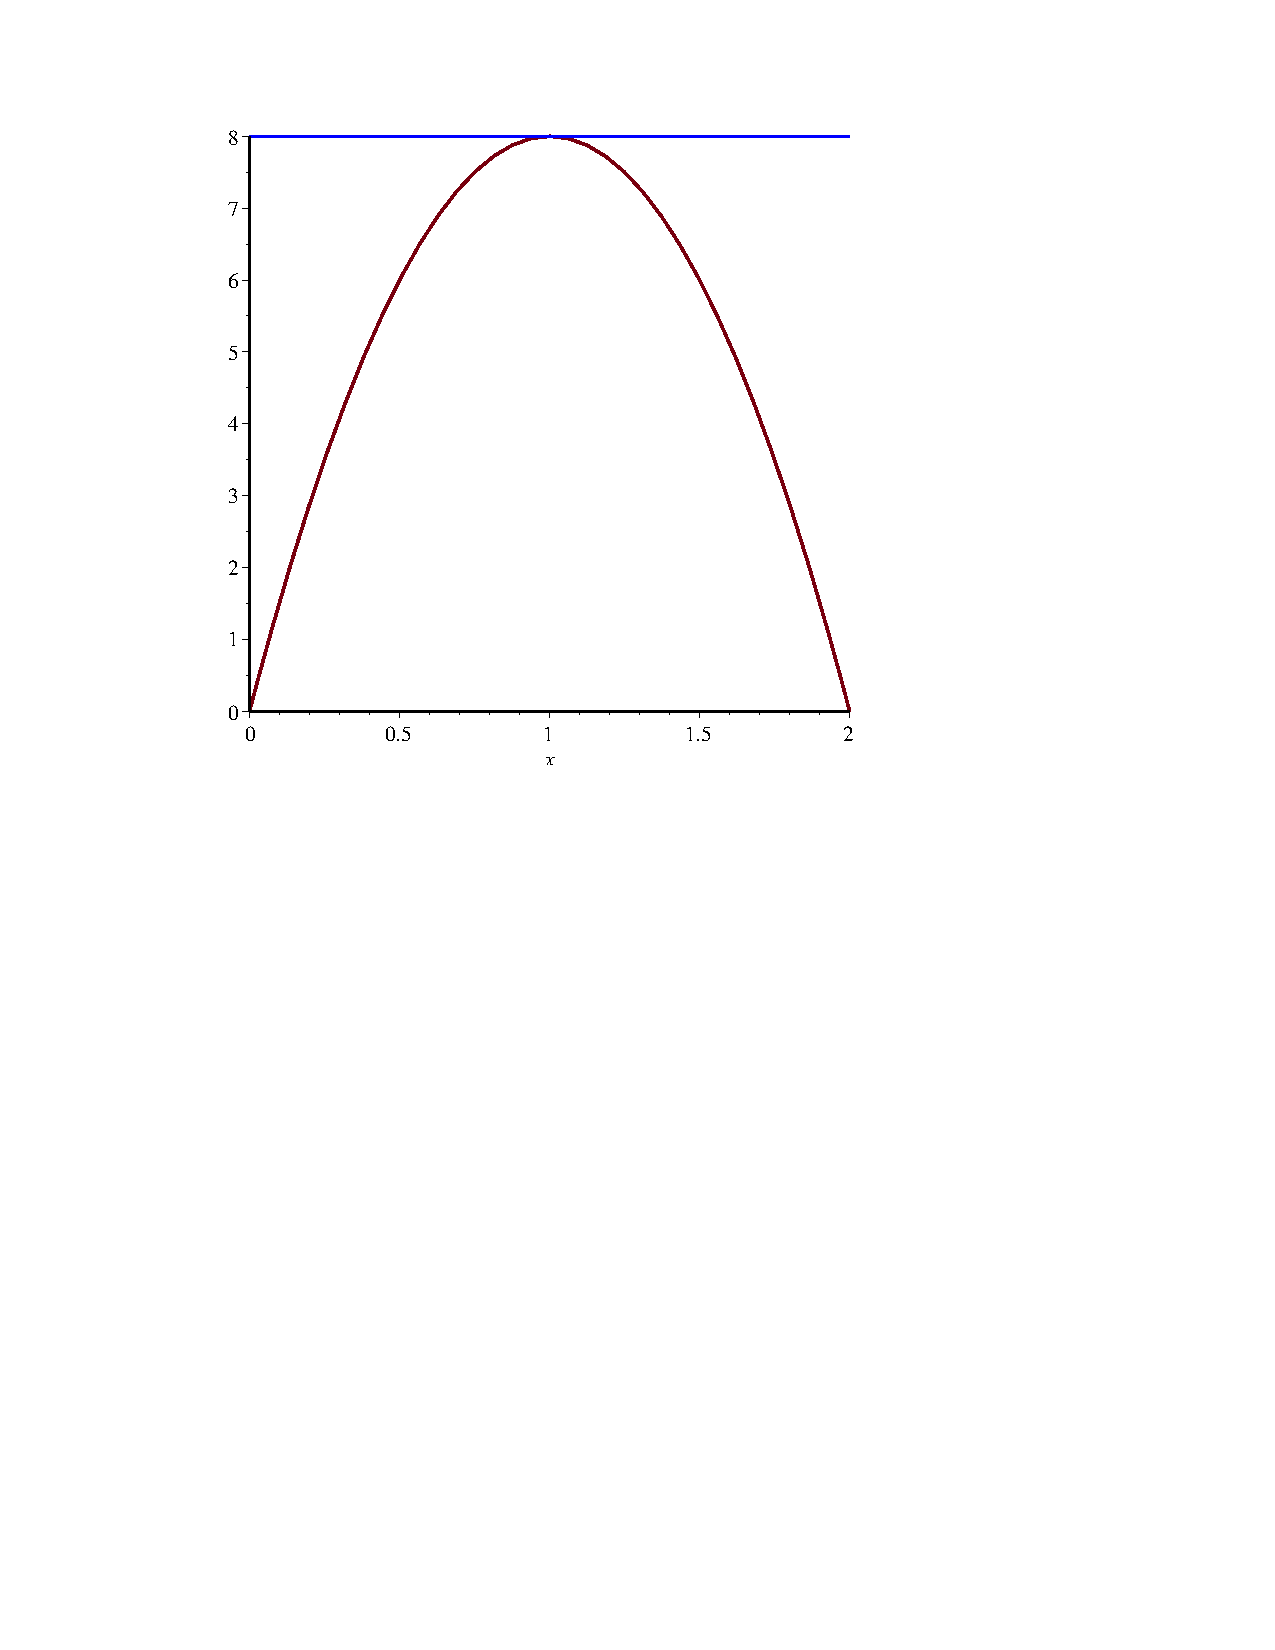
\includegraphics[scale=0.5]{graph4.pdf}}} \fi

\end{enumerate}

\item If a rock is thrown upward on the moon with an initial velocity of 3.244 (m/s), its height (in meters) after $t$ seconds is given by $H(t)=-0.811t^2+3.244t$.

\begin{enumerate}

\item Find the velocity of the rock at $t=a$ seconds.

\ifans{\fbox{$-1.622a+3.244$ m/s}} \fi

\item Find the velocity of the rock at $t=1$ second.

\ifans{\fbox{$1.622$ m/s}} \fi

\item When will the rock hit the surface of the moon?

\ifans{\fbox{At $t=4$ seconds}} \fi

\item Compute the velocity of the rock at the moment when it hits the surface of the moon.

\ifans{\fbox{$-3.244$ m/s}} \fi

\end{enumerate}

\end{enumerate}

\end{document}